\documentclass[12pt]{article}
\usepackage[utf8]{inputenc}
\usepackage[dvips]{graphicx}
\usepackage{epsfig}
\usepackage{fancybox}
\usepackage{verbatim}
\usepackage{array}
\usepackage{latexsym}
\usepackage{alltt}
\usepackage{amssymb}
\usepackage{amsmath}
\usepackage{hyperref}
\usepackage{listings}
\usepackage{color}
\usepackage{algorithm}
\usepackage{algpseudocode}
\usepackage[hmargin=3cm,vmargin=5.0cm]{geometry}
\usepackage{epstopdf}
\graphicspath{ {./images/} }
\usepackage{caption}
\usepackage{tikz}
\usepackage{pgfplots}
\usepackage{multirow}
\topmargin=-1.8cm
\addtolength{\textheight}{6.5cm}
\addtolength{\textwidth}{2.0cm}
\setlength{\oddsidemargin}{0.0cm}
\setlength{\evensidemargin}{0.0cm}
\newcommand{\HRule}{\rule{\linewidth}{1mm}}
\newcommand{\kutu}[2]{\framebox[#1mm]{\rule[-2mm]{0mm}{#2mm}}}
\newcommand{\gap}{ \\[1mm] }
\newcommand{\Q}{\raisebox{1.7pt}{$\scriptstyle\bigcirc$}}
\newcommand{\minus}{\scalebox{0.35}[1.0]{$-$}}



\lstset{
    %backgroundcolor=\color{lbcolor},
    tabsize=2,
    language=MATLAB,
    basicstyle=\footnotesize,
    numberstyle=\footnotesize,
    aboveskip={0.0\baselineskip},
    belowskip={0.0\baselineskip},
    columns=fixed,
    showstringspaces=false,
    breaklines=true,
    prebreak=\raisebox{0ex}[0ex][0ex]{\ensuremath{\hookleftarrow}},
    %frame=single,
    showtabs=false,
    showspaces=false,
    showstringspaces=false,
    identifierstyle=\ttfamily,
    keywordstyle=\color[rgb]{0,0,1},
    commentstyle=\color[rgb]{0.133,0.545,0.133},
    stringstyle=\color[rgb]{0.627,0.126,0.941},
}


\begin{document}

\noindent
\HRule %\\[3mm]
\small
\begin{center}
	\LARGE \textbf{CENG 483} \\[4mm]
	\Large Introduction to Computer Vision \\[4mm]
	\normalsize Spring 2018-2019 \\
	\Large Take Home Exam 3 \\
	\Large Image Colorization \\
    \Large Student Random ID: \\
\end{center}
\HRule

\begin{center}
\end{center}
\vspace{-10mm}
\noindent\\ \\ 
Please fill in the sections below only with the requested information. If you have additional things to mention, you can use the last section. Please note that all of the results in this report should be given for the \textbf{validation set} by default, unless otherwise specified. Also, when you are expected to comment on the effect of a parameter, please make sure to \textbf{fix} other parameters. You may support your comments with visuals (i.e. loss plot).

\section{Baseline Architecture (30 pts)}
    Based on your qualitative results (do not forget to give them),
    \begin{itemize}
        \item Discuss effect of the number of conv layers:
        
		I have fixed the hyperparameters other than number of convolution layers such that kernel size is \textbf{3} except the last convolution layer, number of kernels is \textbf{2} and learning rate is \textbf{0.1}.
		
		\begin{minipage}{\textwidth}
			\begin{minipage}{0.49\textwidth}
				\centering
				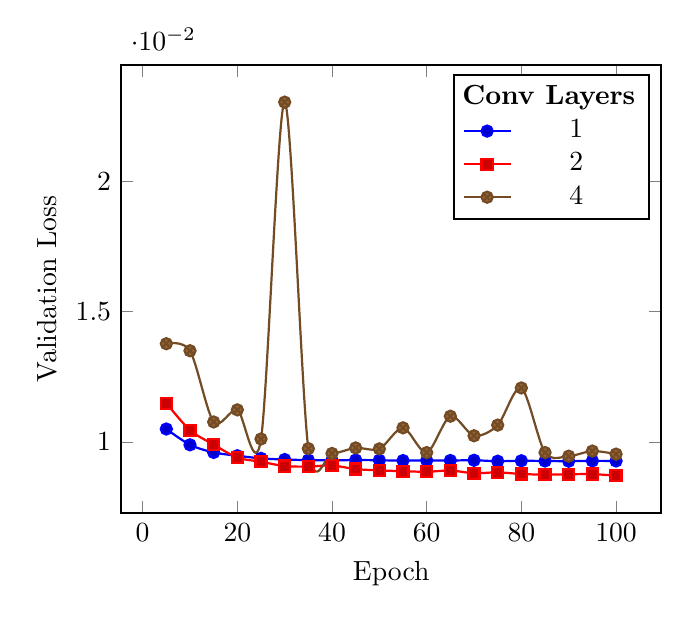
\begin{tikzpicture}
				    \begin{axis}
				        [
				        ,xlabel=Epoch
				        ,ylabel=Validation Loss
				        ,yticklabel style={/pgf/number format/fixed}
				        ,legend style={anchor=north east}
				        ,smooth
				        ,thick
				        ,mark=*
				        ]
   						\addlegendimage{empty legend}
				        \addplot+[smooth] coordinates
				        {(5,0.010491) (10,0.009884) (15,0.009591) (20,0.009465) (25,0.009364) (30,0.009319) (35,0.009298) (40,0.009286) (45,0.009300) (50,0.009291) (55,0.009279) (60,0.009286) (65,0.009282) (70,0.009291) (75,0.009255) (80,0.009272) (85,0.009263) (90,0.009255) (95,0.009268) (100,0.009264)};
				        \addplot+[smooth] coordinates
				        {(5,0.011484) (10,0.010445) (15,0.009895) (20,0.009393) (25,0.009234) (30,0.009068) (35,0.009049) (40,0.009090) (45,0.008953) (50,0.008902) (55,0.008872) (60,0.008849) (65,0.008896) (70,0.008793) (75,0.008827) (80,0.008764) (85,0.008739) (90,0.008753) (95,0.008759) (100,0.008698)};
				        \addplot+[smooth] coordinates
				        {(5,0.013766) (10,0.013496) (15,0.010761) (20,0.011226) (25,0.010108) (30,0.023042) (35,0.009738) (40,0.009552) (45,0.009766) (50,0.009729) (55,0.010536) (60,0.009586) (65,0.010982) (70,0.010232) (75,0.010641) (80,0.012068) (85,0.009587) (90,0.009449) (95,0.009645) (100,0.009527)};
				        \addlegendentry{\hspace{-.7cm}\textbf{Conv Layers}};
   						\addlegendentry{1}
   						\addlegendentry{2}
   						\addlegendentry{4}
				    \end{axis}
				\end{tikzpicture}
				\captionsetup{width=.9\textwidth}
				\captionof{figure}{Validation loss of convolutional neural networks with different number of convolutional layers in the network over 100 epoch}
			 \end{minipage}
			 \hfill
			\begin{minipage}{0.49\textwidth}
				\centering
				\begin{tabular}{ | c | c | }
				  \hline			
				  \bf Convolutional Layers & \bf Validation Loss \\
				  \hline		
				  1 & 0.009255 \\
				  \hline	
				  2 & 0.008698 \\
				  \hline	
				  4 & 0.009449 \\
				  \hline
				\end{tabular}
				\captionsetup{width=.8\textwidth}
				\captionof{table}{The lowest validation losses of convolutional neural networks achieved with different number of convolutional layers in the network}
			\end{minipage}
		\end{minipage} \\
		        
        \item Discuss effect of the kernel size(except the last conv layer):
        
		I have fixed the hyperparameters other than kernel size such that the number of convolutional layer is \textbf{2}, the number of kernels is \textbf{2} and learning rate is \textbf{0.1}.
		
		\begin{minipage}{\textwidth}
			\begin{minipage}{0.49\textwidth}
				\centering
				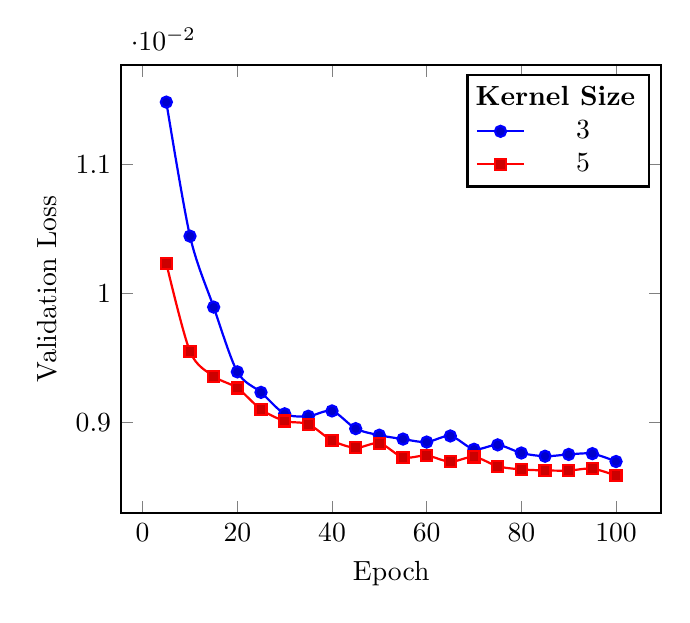
\begin{tikzpicture}
				    \begin{axis}
				        [
				        ,xlabel=Epoch
				        ,ylabel=Validation Loss
				        ,yticklabel style={/pgf/number format/fixed}
				        ,legend style={anchor=north east}
				        ,smooth
				        ,thick
				        ,mark=*
				        ]
   						\addlegendimage{empty legend}
				        \addplot+[smooth] coordinates
				        {(5,0.011484) (10,0.010445) (15,0.009895) (20,0.009393) (25,0.009234) (30,0.009068) (35,0.009049) (40,0.009090) (45,0.008953) (50,0.008902) (55,0.008872) (60,0.008849) (65,0.008896) (70,0.008793) (75,0.008827) (80,0.008764) (85,0.008739) (90,0.008753) (95,0.008759) (100,0.008698)};
				        \addplot+[smooth] coordinates
				        {(5,0.010234) (10,0.009551) (15,0.009359) (20,0.009268) (25,0.009102) (30,0.009012) (35,0.008987) (40,0.008861) (45,0.008804) (50,0.008840) (55,0.008730) (60,0.008744) (65,0.008696) (70,0.008734) (75,0.008661) (80,0.008637) (85,0.008629) (90,0.008628) (95,0.008643) (100,0.008588)};
				        \addlegendentry{\hspace{-.7cm}\textbf{Kernel Size}};
   						\addlegendentry{3}
   						\addlegendentry{5}
				    \end{axis}
				\end{tikzpicture}
				\captionsetup{width=.9\textwidth}
				\captionof{figure}{Validation loss of convolutional neural network with different kernel sizes over 100 epoch}
			 \end{minipage}
			 \hfill
			\begin{minipage}{0.49\textwidth}
				\centering
				\begin{tabular}{ | c | c | }
				  \hline			
				  \bf Kernel Size & \bf Validation Loss \\
				  \hline		
				  3 & 0.008698 \\
				  \hline	
				  5 & 0.008588 \\
				  \hline
				\end{tabular}
				\captionsetup{width=.8\textwidth}
				\captionof{table}{The lowest validation losses of convolutional neural networks achieved with different kernel sizes}
			\end{minipage}
		\end{minipage} \\
        
        \item Discuss effect of the number of kernels(except the last conv layer):
        
        I have fixed the hyperparameters other than the number of kernels (except the last convolutional layer) such that the number of convolutional layer is \textbf{2}, kernel size is \textbf{5} and learning rate is \textbf{0.1}.
        
		\begin{minipage}{\textwidth}
			\begin{minipage}{0.49\textwidth}
				\centering
				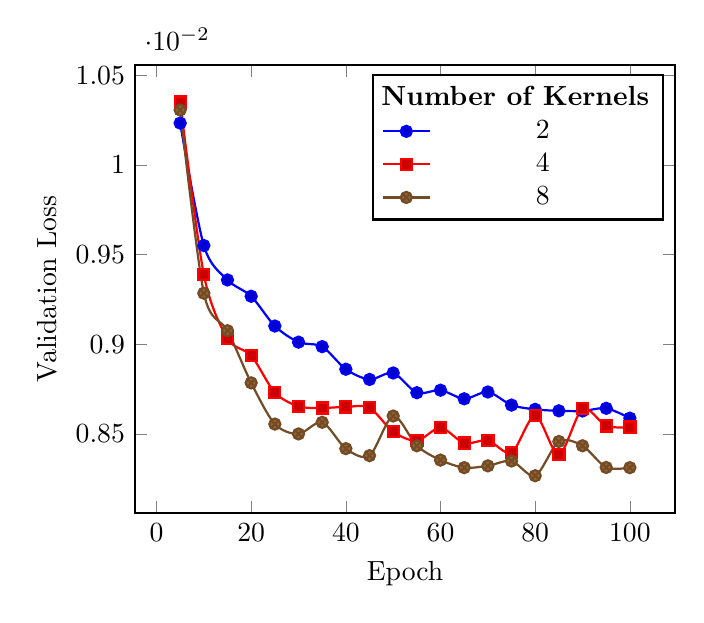
\begin{tikzpicture}
				    \begin{axis}
				        [
				        ,xlabel=Epoch
				        ,ylabel=Validation Loss
				        ,yticklabel style={/pgf/number format/fixed}
				        ,legend style={anchor=north east}
				        ,smooth
				        ,thick
				        ,mark=*
				        ]
   						\addlegendimage{empty legend}
				        \addplot+[smooth] coordinates
				        {(5,0.010234) (10,0.009551) (15,0.009359) (20,0.009268) (25,0.009102) (30,0.009012) (35,0.008987) (40,0.008861) (45,0.008804) (50,0.008840) (55,0.008730) (60,0.008744) (65,0.008696) (70,0.008734) (75,0.008661) (80,0.008637) (85,0.008629) (90,0.008628) (95,0.008643) (100,0.008588)};
				        \addplot+[smooth] coordinates
				        {(5,0.010351) (10,0.009389) (15,0.009033) (20,0.008937) (25,0.008731) (30,0.008654) (35,0.008645) (40,0.008651) (45,0.008646) (50,0.008512) (55,0.008462) (60,0.008535) (65,0.008449) (70,0.008464) (75,0.008396) (80,0.008602) (85,0.008385) (90,0.008640) (95,0.008545) (100,0.008538)};
				        \addplot+[smooth] coordinates
				        {(5,0.010307) (10,0.009285) (15,0.009076) (20,0.008785) (25,0.008555) (30,0.008500) (35,0.008565) (40,0.008418) (45,0.008379) (50,0.008600) (55,0.008434) (60,0.008354) (65,0.008312) (70,0.008322) (75,0.008349) (80,0.008267) (85,0.008458) (90,0.008434) (95,0.008313) (100,0.008312)};
				        \addlegendentry{\hspace{-.7cm}\textbf{Number of Kernels}};
   						\addlegendentry{2}
   						\addlegendentry{4}
   						\addlegendentry{8}
				    \end{axis}
				\end{tikzpicture}
				\captionsetup{width=.9\textwidth}
				\captionof{figure}{Validation loss of convolutional neural networks with different number of kernels over 100 epoch}
			 \end{minipage}
			 \hfill
			\begin{minipage}{0.49\textwidth}
				\centering
				\begin{tabular}{ | c | c | }
				  \hline			
				  \bf The Number of Kernels & \bf Validation Loss \\
				  \hline		
				  2 & 0.008588 \\
				  \hline	
				  4 & 0.008385 \\
				  \hline	
				  8 & 0.008267 \\
				  \hline
				\end{tabular}
				\captionsetup{width=.8\textwidth}
				\captionof{table}{The lowest validation losses of convolutional neural networks achieved with different number of kernels}
			\end{minipage}
		\end{minipage} \\
        
        \item Discuss effect of the learning rate by choosing three values: a very large one, a very small one and a value of your choice:
        
        I have fixed the hyperparameters other than the learning rate such that the number of convolutional layer is \textbf{2}, kernel size is \textbf{5} and the number of kernels is \textbf{8}.

		\begin{minipage}{\textwidth}
			\begin{minipage}{0.49\textwidth}
				\centering
				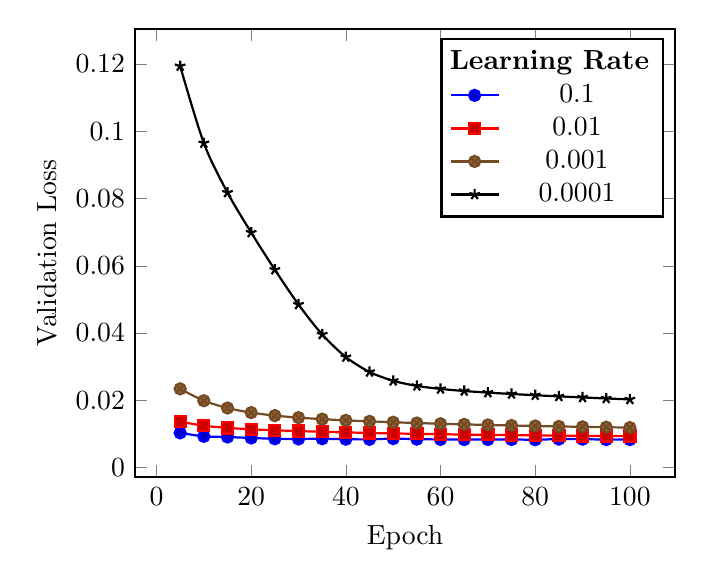
\begin{tikzpicture}
				    \begin{axis}
				        [
				        ,xlabel=Epoch
				        ,ylabel=Validation Loss
				        ,yticklabel style={/pgf/number format/fixed}
				        ,legend style={anchor=north east}
				        ,smooth
				        ,thick
				        ,mark=*
				        ]
   						\addlegendimage{empty legend}
				        \addplot+[smooth] coordinates
				        {(5,0.010307) (10,0.009285) (15,0.009076) (20,0.008785) (25,0.008555) (30,0.008500) (35,0.008565) (40,0.008418) (45,0.008379) (50,0.008600) (55,0.008434) (60,0.008354) (65,0.008312) (70,0.008322) (75,0.008349) (80,0.008267) (85,0.008458) (90,0.008434) (95,0.008313) (100,0.008312)};
				        \addplot+[smooth] coordinates
				        {(5,0.013659) (10,0.012425) (15,0.011799) (20,0.011369) (25,0.011075) (30,0.010833) (35,0.010627) (40,0.010452) (45,0.010283) (50,0.010142) (55,0.010016) (60,0.009923) (65,0.009792) (70,0.009722) (75,0.009640) (80,0.009557) (85,0.009482) (90,0.009408) (95,0.009357) (100,0.009342)};
				        \addplot+[smooth] coordinates
				        {(5,0.023399) (10,0.019873) (15,0.017698) (20,0.016331) (25,0.015445) (30,0.014838) (35,0.014389) (40,0.014032) (45,0.013732) (50,0.013470) (55,0.013235) (60,0.013022) (65,0.012832) (70,0.012658) (75,0.012501) (80,0.012356) (85,0.012223) (90,0.012100) (95,0.011987) (100,0.011880)};
				        \addplot+[smooth] coordinates
				        {(5,0.119384) (10,0.096475) (15,0.081766) (20,0.069889) (25,0.058836) (30,0.048486) (35,0.039583) (40,0.032862) (45,0.028430) (50,0.025795) (55,0.024286) (60,0.023379) (65,0.022762) (70,0.022283) (75,0.021874) (80,0.021504) (85,0.021162) (90,0.020844) (95,0.020545) (100,0.020264)};
				        \addlegendentry{\hspace{-.7cm}\textbf{Learning Rate}};
   						\addlegendentry{0.1}
   						\addlegendentry{0.01}
   						\addlegendentry{0.001}
   						\addlegendentry{0.0001}
				    \end{axis}
				\end{tikzpicture}
				\captionsetup{width=.9\textwidth}
				\captionof{figure}{Validation loss of convolutional neural networks with different learning rates over 100 epoch}
			 \end{minipage}
			 \hfill
			\begin{minipage}{0.49\textwidth}
				\centering
				\begin{tabular}{ | c | c | }
				  \hline			
				  \bf Learning Rate & \bf Validation Loss \\
				  \hline		
				  0.1 & 0.008267 \\
				  \hline	
				  0.01 & 0.009342 \\
				  \hline	
				  0.001 & 0.011880 \\
				  \hline
				  0.0001 & 0.020264 \\
				  \hline
				\end{tabular}
				\captionsetup{width=.8\textwidth}
				\captionof{table}{The lowest validation losses of convolutional neural networks achieved with different learning rates}
			\end{minipage}
		\end{minipage} \\

    \end{itemize}


\section{Further Experiments (20 pts)}
    Based on your qualitative results (do not forget to give them),
    \begin{itemize}
        \item Try adding a batch-norm layer (torch.nn.BatchNorm2d) into each convolutional layer. How does it affect the results, and, why? Keep it if it is beneficial. 
        
        \item Try adding a tanh activation function after the very last convolutional layer. How does it affect the results, and, why? Keep it if it is beneficial. 
        
        \item Try setting the number of channels parameter to 8. How does it affect the results, and, why? Keep it if it is beneficial. 
        
      
    \end{itemize}


\section{Your Best Configuration (20 pts)}
Using the best model that you obtain, report the following:
 
    \begin{itemize}
        \item The automatically chosen number of epochs(what was your strategy?):
        \item The plot of the training mean-squared error loss over epochs:
        \item The  plot  of  the  validation  12-margin  error  over  epochs (see the3 text for details):
        \item At least 5 qualitative results on the validation set, showing the prediction and the target colored image:
        \item Discuss the advantages and disadvantages of the model, based on your qualitative results, and, briefly discuss potential ways to improve the model:
    \end{itemize}
    
\section{Your Results on the Test Set(30 pts)}
This part will be obtained by us using the estimations you will provide. Please tell us how should we run your code in case of a problem:

\section{Additional Comments and References}

    (if there any)





\end{document}


